\chapter{Aerodynamic Analysis}
\label{ch:Aerodynamic_Analysis}
In this chapter, the aerodynamic properties of the entire aircraft in cruise will be assessed.
First, in \Cref{sec:DRAG}, the drag will be analysed, after which the aerodynamics of the full parametric model will be studied in \Cref{sec:AeroBuildup}, and both will be verified and validated in \Cref{sec:vv_aero}

\section{Drag}
\label{sec:DRAG}
% While XFLR5 is an excellent tool for modeling the wing and empennage and comparing various geometric parameters, its drag polar does not accurately reflect the drag for the entire UAV. This discrepancy arises because the UAV's drag is significantly influenced by elements such as the fuselage shape, rotors, and landing gear, which XFLR5 cannot model precisely. Therefore, a more detailed drag estimation is required for a comprehensive understanding of the drag contributions. For this purpose, Raymer's component buildup method is employed, a standard technique in aircraft design, also used for similar VTOL UAV configurations. Unless otherwise noted, the equations and data for constructing the drag polar are sourced from Raymer's book.

Drag consists of lift-induced drag and parasite drag, with the latter mainly depending on the shape and interaction of various UAV components.
Unless explicitly stated otherwise, all formulas and statements in this section are from the Raymer book~\cite{raymer1992aircraft}.
The drag polar is defined by the following equation:

\begin{equation}
    C_D = C_{D0} + \frac{C_L^2}{\pi \mathrm{AR} e}
\end{equation}
 

Here, $C_D$ is the total drag coefficient, 
$C_{D0}$ is the zero-lift drag coefficient, $C_L$ is the lift coefficient, $\mathrm{AR}$ is the aspect ratio of the main wing, and $e$ is the Oswald efficiency factor.
The parasite, or zero-lift, drag can be further broken down using the component build-up method from Raymer \cite{raymer1992aircraft}:

\begin{equation}
    C{D_0} = \frac{\sum C_{f_{c}} \mathrm{FF}_C Q_C S_\text{wet,c}}{S_\text{ref}} + C_{D_\text{misc}} + C_{D_{L\&P}}
\end{equation}

Where the subscript c denotes the component and the other parameters are defined as follows:

\begin{itemize}
    \item $C_f$: Flat-plate skin-friction drag coefficient.
    \item $\mathrm{FF}$: Form factor related to pressure drag from viscous separation.
    \item $Q$: Interference factor
    \item $S_\text{wet}$: Wetted surface area, exposed to air
    \item $S_\text{ref}$: Reference surface area, the wing’s projected area.
    \item $C_{D_\text{misc}}$: Miscellaneous drag from special features
    \item $C_{D_{L\&P}}$: Drag from leaks and protuberances
\end{itemize}

The different components will be assessed for each parameter, and after that, they will be summed up.
This allows for determining the miscellaneous drag and drag from leaks and protuberances, which will be added to obtain the zero-lift drag coefficient.
The four subsystems that will be considered are the wing, fuselage, empennage and the nacelles.
Due to the iterative nature of the drag, the design of the empennage will be further discussed in \Cref{ch:Stability_and_Control}, and the nacelles will be further discussed in \Cref{ch:Propulsion}.
Furthermore, it is important to state that all variables given in the tables in this section are the variables after the entire aeroplane has been integrated and converged.

\subsubsection{Flat-Plate Skin-Friction Coefficient}
The flat-plate skin-friction coefficient differs for laminar and turbulent flow, calculated using the following equations for laminar and turbulent cases, respectively:

\noindent\begin{minipage}[H]{.5\linewidth}
\begin{equation}
    R = \frac{\rho V l}{\mu}
\end{equation}
\end{minipage}%
\begin{minipage}{.5\linewidth}
\begin{equation}
    C_{f_{laminar}} = \frac{1.328}{R}
\end{equation}
\end{minipage}

\begin{equation}
    C_{f_{turbulent}} = \frac{0.455}{(\log_{10}R)^{2.58} (1+0.144M^2)^{0.65}}
\end{equation}

Here, $M$ is the Mach number, $\rho$ is air density, $V$ is free stream velocity, $l$ is characteristic length, and $\mu$ is kinematic viscosity.
The overall skin friction coefficient is the weighted average of laminar and turbulent cases, requiring an estimation of the laminar flow portion.
Since the fuselage has a tadpole shape and is composite, around 25\% of the fuselage has laminar flow, and the wing and tail surfaces can achieve about 40\% laminar flow.
With all this information, the flat-plate skin-friction coefficient for each of the four subsystems can be calculated, and the values used and final values can be found in \Cref{tab:Skin-Friction_coefficient}.

\begin{table}[H]
    \centering
    \caption{Skin friction coefficient values}
    \label{tab:Skin-Friction_coefficient}
    \begin{tabular}{
        l|
        S[table-format=2.2]
        S[table-format=2]
        S[table-format=1.5, parse-numbers=false]
        S[table-format=1.4, parse-numbers=false]
        S[table-format=1.4, parse-numbers=false]
    }
        \toprule
        \textbf{Group}       & \textbf{Reynolds Number} [\num{1e6}]  & \textbf{Laminar} [\unit{\%}] & \textbf{$C_{f_\text{lam}}$} [{-}] & \textbf{$C_{f_\text{tur}}$} [{-}] & \textbf{$C_f$} [{-}] \\ \midrule
        Wing        & 4.00                  &  40        & 0.00067      & 0.0035 & 0.0023         \\
        Fuselage    & 28.5               &  25        & 0.00024      & 0.0025 & 0.0020          \\
        Empennage   & 4.50                &  40        & 0.00061      & 0.0034 & 0.0023          \\
        Nacelles    & 4.75               &  0         & 0.00060      & 0.0034 & 0.0034 \\
        \bottomrule
    \end{tabular}
\end{table}

\subsubsection{Form Factor}

The form factor for wings and empennage is calculated using the following equation.

\begin{equation}
\left.\mathrm{FF}=\left[1+\frac{0.6}{(x / c)_m}\left(\frac{t}{c}\right)+100\right)\left(\frac{t}{c}\right)^4\right]\left[1.34 M^{0.18}\left(\cos \Lambda_m\right)^{0.28}\right]
\end{equation}

Where $(t/c)$ is the maximum thickness-to-chord ratio
and $(x/c)_m$ is the position where this maximum ratio is found along the chord.
$M$ is the Mach number, and $\Lambda_m$ the sweep of the maximum thickness line.
The form factor considering the fuselage and nacelle would conclude the following equations, leading to the resultant values in \Cref{tab:Form Factor}.

\begin{minipage}[H]{.5\linewidth}
\begin{equation}
    \mathrm{FF}_\text{fuselage}=\left(1+\frac{60}{f^3}+\frac{f}{400}\right)
\end{equation}
\end{minipage}%
\begin{minipage}{.5\linewidth}
\begin{equation}
    \mathrm{FF}_\text{nacelle} = 1 + (0.35/f)
\end{equation}
\end{minipage}\\
where:
\begin{equation}
    f = \frac{l}{d}
\end{equation}

\begin{table}[H]
    \centering
    \caption{Form factor values}
    \label{tab:Form Factor}
    \begin{tabular}{l|S[table-format=1.2]}
        \toprule
        \textbf{Group}       & \textbf{Form Factor} [{-}]      \\ \midrule
        Wing        & 1.45             \\
        Fuselage    & 1.58             \\
        Empennage   & 1.45             \\
        Nacelles    & 1.07             \\\bottomrule
    \end{tabular}
\end{table}



\subsubsection{Interference Factor}
The interference factor describes component interference, which adds drag and is estimated as follows:
\begin{itemize}
    \item $Q_\text{wing}$ = 1.0 for a high-wing configuration.
    \item $Q_\text{fuselage}$ = 1.0, as it also has negligible interference.
    \item $Q_\text{tail}$ = 1.03, for a smooth V-tail,
    \item $Q_\text{nacelle}$ = 1.3, since the nacelle is less than one diameter from the wing.
\end{itemize}
 
\subsubsection{Wetted Surface Area}
Finally, the wetted surface area for each component is defined as the \Cref{tab:Wetted Surface Area}.

\begin{table}[H]
    \centering
    \caption{Wetted surface area values}
    \label{tab:Wetted Surface Area}
    \begin{tabular}{l|S[table-format=2.1]}
        \toprule
        \textbf{Group}       & \textbf{$S_\text{wet}$} [\unit{m^2}]      \\ \midrule
        Wing        & 24.9             \\
        Fuselage    & 24.6             \\
        Empennage   & 9.9             \\
        Nacelles    & 1.9             \\
        \bottomrule
    \end{tabular}
\end{table}


 
\subsubsection{Miscellaneous, Leak, and Protuberances Drag}
These types of drag consider the whole aircraft and are therefore not calculated with the component buildup method but rather defined as a percentage of the sum of the component buildup method.
The only component that has not yet been considered for miscellaneous drag is the landing gear.
The landing gear will be discussed more in-depth in \Cref{ch:Structures_and_Materials}, but for now, based on literature and the design, it is assumed that the landing gear will add 3\% to the $C_{D_0}$ of the component build-up method.
Leaks and protuberance drag are more difficult to predict.
With enough care, the protuberance drag can also be reduced to nearly zero, but at a considerable expense.
Since the \textit{Swing} is made mainly of composites and therefore does not have rivets or skin panels, it has little protuberance drag, but because of the hinge mechanism, the protuberance drag increases again.
The hinge mechanism will also cause more leakage drag.
For general aviation aircraft, the leakage and protuberance drag can be estimated to be between 2–5\% and for fighters this is between 5–10\%.
To account for the hinge in the design and taking into account the fact that the \textit{Swing} is made from composites, the drag due to leakage and protuberance is assumed to be 12\% of the $C_{D_0}$ of the component build-up.
Therefore, the total increase due to miscellaneous and L\&P drag is 15\%
 
\subsubsection{Total Parasite Drag}
\begin{table}[H]
    \centering
    \caption{Parasite drag values}
    \label{tab:Parasite-Drag}
    \sisetup{exponent-mode=fixed}
    \begin{tabular}{l|S|S|S|S|S|S|S} \toprule
        \textbf{Component}      & \textbf{$C_f$}  &  \textbf{$\mathrm{FF}$}  &  \textbf{$Q$}   & \textbf{$S_\text{wet}$}   &  \textbf{$C_{D_0},c$} & \textbf{$C_{D_\text{Misc, L\&P}}$} &\\ \midrule
        Wing           & 0.0023 &  1.45  &  1.0   &  24.9 &     0.0024          & &\\
        Fuselage       & 0.0020 &  1.58  &  1.0   &  24.6 &     0.0061          & &\\
        Empennage      & 0.0023 &  1.45  &  1.03  &  9.9  &     0.0054          & &\\
        Nacelles       & 0.0034 &  1.07  &  1.3   &  1.9  &     0.0039          & &\\ \midrule
        \textbf{Sum}   &       &         &        &       &     \textbf{0.0179} & 0.0026 &\\  \midrule
        \textbf{$C_{D_0}$}   &       &       &       &    &                     & &   \textbf{0.0206}              \\  \bottomrule
    \end{tabular}
\end{table}

\subsection{Lift Induced Drag}
The lift-induced drag is only dependent on the wing shape, which has been defined in \Cref{ch:AerodynamicDesign}.
The lift-induced drag is defined by:
\begin{equation}
    C_{D_\text{ind}}=\frac{C_L^2}{\pi \mathrm{AR} e}
\end{equation}
Where $\mathrm{AR}$ is the aspect ratio, which is 14, $C_L$ is the lift coefficient, and $e$ is the Oswald efficiency factor, defined by \Cref{eq:Oswald}:
\begin{equation}
\label{eq:Oswald}
e=1.78\left(1-0.045 \mathrm{AR}^{0.68}\right)-0.64
\end{equation}
which gives an efficiency factor of \num{0.658}.
With these values, the drag as a function of lift, also known as the drag polar, can be computed, which can be seen in \Cref{fig:AeroValidationPlots}:

\section{Aerodynamics of Full Parametric Model}\label{sec:AeroBuildup}
To improve the understanding of the aerodynamics of the aircraft,
a full parametric model of the \textit{Swing} was constructed and analysed using the AeroSandbox tool~\cite{aerosandbox}.
The parametric model was constructed using the dimensions and properties of the \textit{Swing} as defined in the previous chapters.
It is displayed in \Cref{fig:AeroSandboxModel}.

\begin{figure}[ht]
    \centering
    
\includegraphics[width=0.7\linewidth]{figures/AerodynamicAnalysis/rotating_wing_three_view}
    \caption{Three-view of the parametric model of the \textit{Swing eVTOL}}
    \label{fig:AeroSandboxModel}
\end{figure}

For the aerodynamic analysis, the AeroBuildup Aerodynamics Engine in AeroSandbox was used.
It is designed for conceptual design and preliminary design of aircraft, and is based on the USAF DATCOM methodology~\cite{DATCOM}.
It computes aerodynamic forces, moments, and stability derivatives, modelling viscous and compressible effects on wings and fuselages across any orientation and arbitrary angular rates.
Using the engine proved to be invaluable in the design process,
as it allowed for a more detailed analysis of the aerodynamic properties across a wider range of conditions than the class II estimation.

In addition to the engine's base functionality,
AeroBuildup has been extended to include the ability to model the aerodynamic properties of rotating wings.
Also, a method was added to compute the stability derivatives with respect to elevator and aileron deflections.
This was done by changing the parametric model to include control surfaces and then computing the aerodynamic forces for different deflections of the control surfaces.
The stability derivatives were then computed by fitting the aerodynamic forces to a linear model.
The results of the stability derivatives are shown in \Cref{tab:stability_coefficients}.

\begin{table}[ht]
    \centering
    \caption{Stability coefficients of the \textit{Swing} for $\alpha=0$, $\beta=0$, $\delta_e=0$, $\delta_a=0$, and $V=$\qty{200}{\km\per\hour}}
    \label{tab:stability_coefficients}
    \sisetup{table-format=+2.4, round-mode=figures, round-precision=3}
    \begin{tabular}{@{}lS|lS@{}}
        \toprule
        \multicolumn{2}{c|}{\textbf{Forces}} & \multicolumn{2}{c}{\textbf{Moments}} \\
        \midrule
        $C_{X_\alpha}$ & 0.5908323618541962 & $C_{l_\beta}$ & -0.007935486607432665 \\
        $C_{X_{\delta_e}}$ & -0.03407082 & $C_{l_{\dot{beta}}}$ & 0.02868203930519337 \\
        $C_{X_u}$ & -0.0711051970171767 & $C_{l_{\delta_a}}$ & -0.75240091 \\
        $C_{Y_\beta}$ & -0.44100361489142725 & $C_{l_p}$ & -0.5373051886812819 \\
        $C_{Y_{\dot{\beta}}}$ & 0.06394017232712843 & $C_{l_r}$ & 0.11381761629044988 \\
        $C_{Y_{\delta_a}}$ & -0.18953364 & $C_{m_\alpha}$ & -1.6001123621538174 \\
        $C_{Y_p}$ & -0.06598204721386793 & $C_{m_{\dot{\alpha}}}$ & 0.6995033722413452 \\
        $C_{Y_r}$ & 0.25373084256796996 & $C_{m_{\delta_e}}$ & -5.11807994 \\
        $C_{Z_0}$ & -0.6392443102725556 & $C_{m_q}$ & -36.61930046989947 \\
        $C_{Z_\alpha}$ & -6.886773821818554 & $C_{n_\beta}$ & 0.01271770096349569 \\
        $C_{Z_{\dot{\alpha}}}$ & -0.05018096210843948 & $C_{n_{\dot{\beta}}}$ & -0.01661455255 \\
        $C_{Z_{\delta_e}}$ & -1.32378707 & $C_{n_{\delta_a}}$ & -0.00426444 \\
        $C_{Z_q}$ & -2.626994811232408 & $C_{n_p}$ & -0.09154303879909277 \\
        $C_{Z_u}$ & -1.4632708658248335 & $C_{n_r}$ & -0.0659307640988797 \\
        \bottomrule
    \end{tabular}
\end{table}


\section{Verification and Validation}
\label{sec:vv_aero}
To verify the drag polar, the zero-lift drag components have been hand-calculated for a single iteration of the aircraft.
Initially, some values did not match when rounded to three significant digits.
For instance, the tail was not within three decimals of the result from the model, which turned out to be due to a wrong assumption about the tail area.
Furthermore, the AeroSandbox tool was used to analyse the aerodynamic properties of the \textit{Swing} as explained in \Cref{sec:AeroBuildup}.
A comparison was made between the AeroSandbox and the class II estimation. As can be seen in \Cref{fig:AeroValidationPlots},
they are similar for an $\alpha$ range between -5 and 10 degrees, after which it starts to divert.
The main difference in drag polar is for high negative lift, but it is not crucial since the aircraft will not fly in a negative lift.

Also, the custom methods in the aerodynamic engine from \Cref{sec:AeroBuildup} are validated by comparing the results with data from the Cessna 172 aircraft.
The stability coefficients had the same sign and order of magnitude as the Cessna 172, which is a good indication that the custom methods are working correctly.
Some deviations are found,
but these are expected due to the differences in the aircraft’s design, for instance, the large tail of the \textit{Swing} compared to the Cessna 172.

\begin{figure}[h]
    \centering
    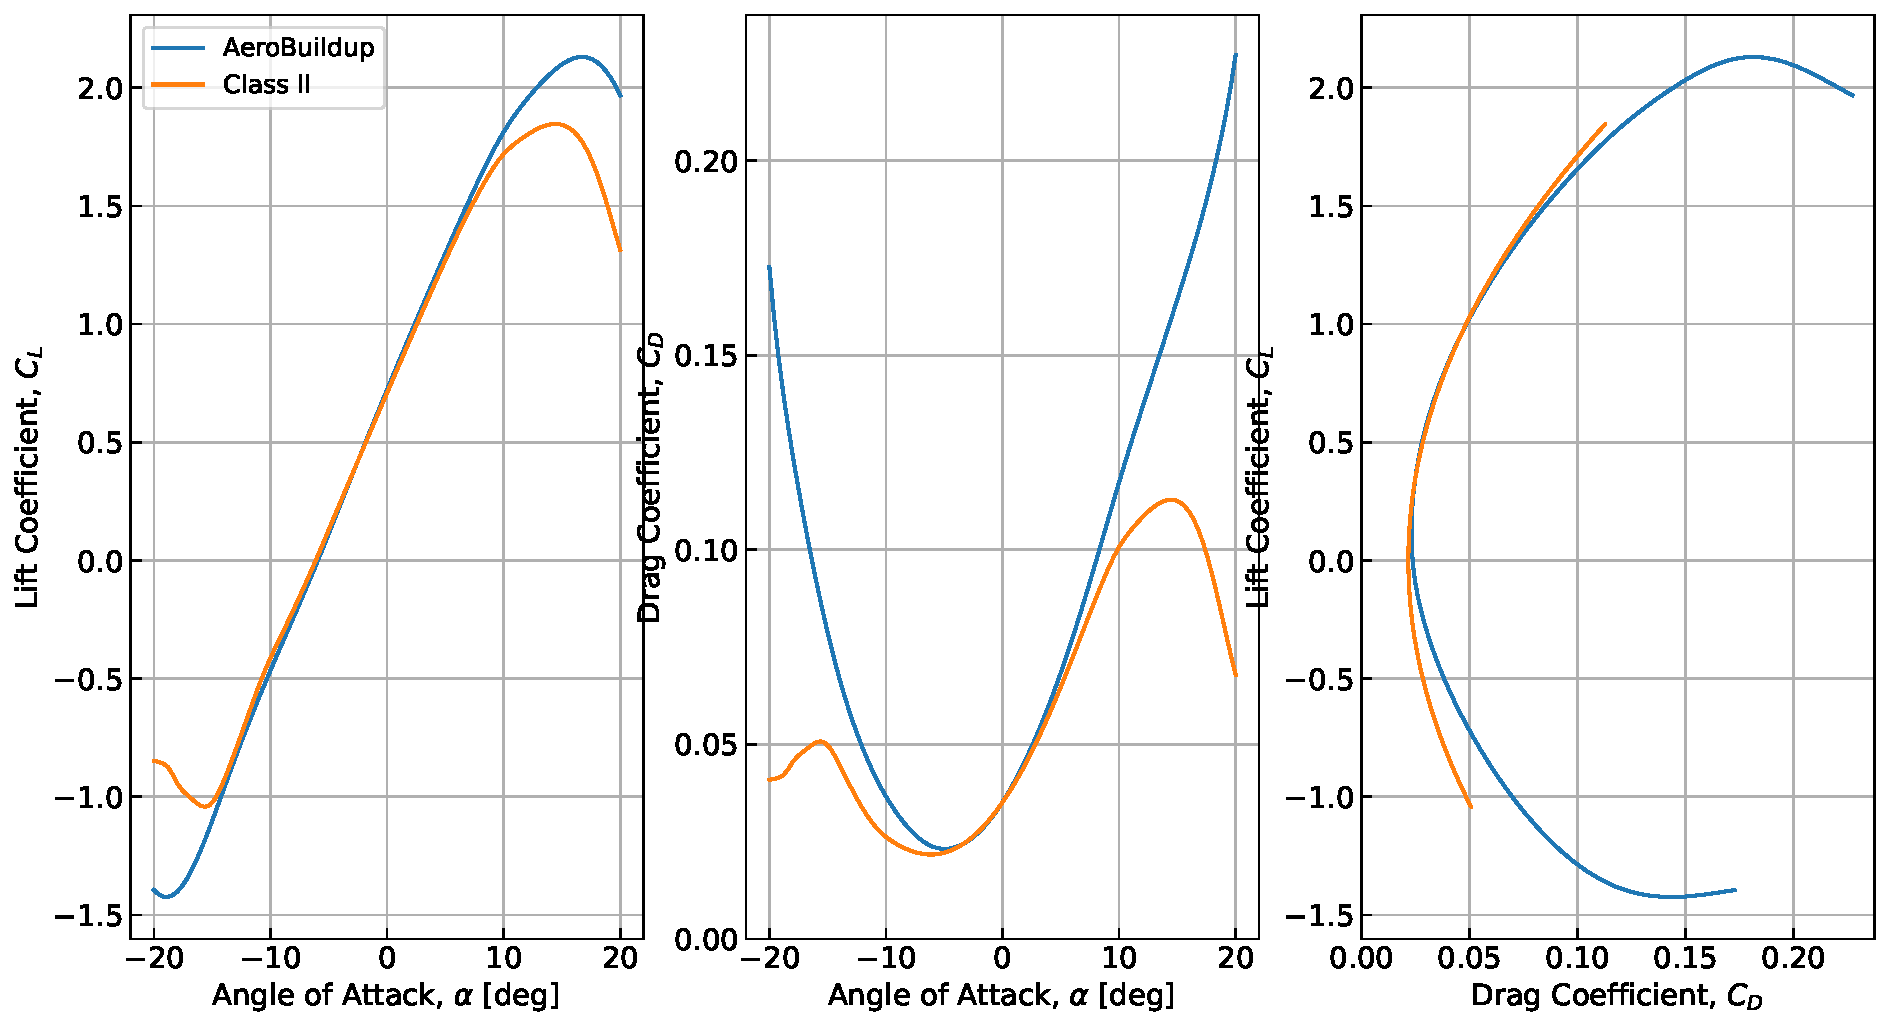
\includegraphics[width=0.9\linewidth]{figures/AerodynamicAnalysis/Aero_validation_plots}
    \caption{Comparison of the lift and drag polars between the class II estimation and the AeroSandbox model}
    \label{fig:AeroValidationPlots}
\end{figure}

